\section{Implementierung}
In diesem Kapitel wollen wir auf die Implementierung unseres Prototypen eingehen.


\subsection{Vorstellung des Ablaufs}
Zunächst beschreiben wir dazu den grundsätzlichen Ablauf des Prozesses anhand einer Skizze:
\begin{figure}[H]
\centering
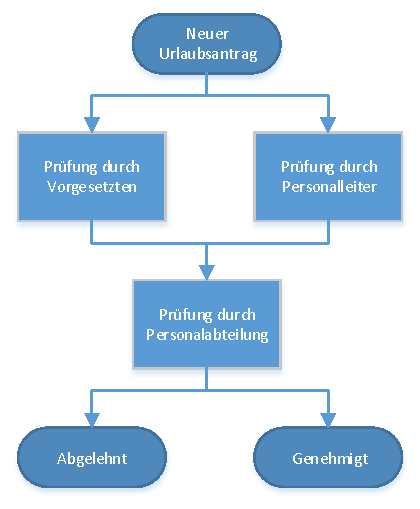
\includegraphics[width=0.5\linewidth]{Bilder/Workflow}
\caption{Skizze des Prozessablaufs}
\label{fig:Workflow}
\end{figure}

Hat ein Mitarbeiter einen Urlaubsantrag ausgefüllt startet ein neuer Urlaubsgenehmigungsprozess. Der Antrag muss an verschiedenen Stellen geprüft werden. In unserem Beispielunternehmen muss der Urlaubsantrag durch den Vorgesetzten und ggf. dem Leiter der Personalabteilung genehmigt werden. Da die Reihenfolge hierbei keine Rolle spielt, können die beiden Schritte parallel ausgeführt werden. Abschließend prüft die Personalabteilung, ob der Mitarbeiter noch über genügend freie Urlaubstage verfügt und genehmigt bzw. verweigert den Antrag.	
	
	
\subsection{Systemübersicht}

\begin{figure}[H]
\centering
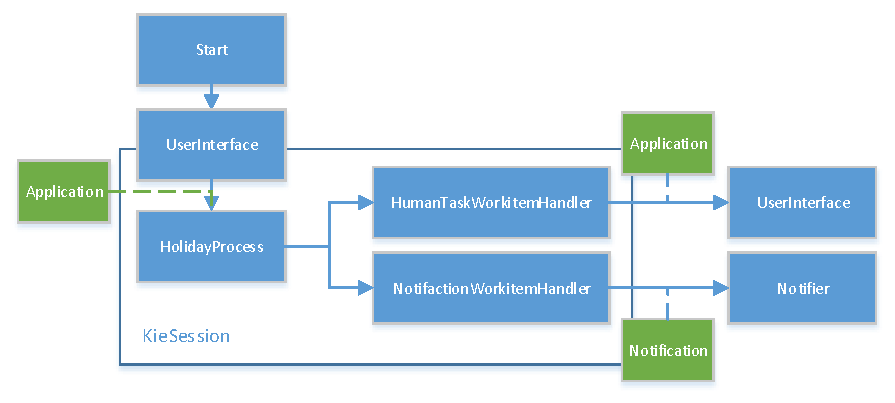
\includegraphics[width=1.0\linewidth]{Bilder/Komponenten}
\caption{Eine Übersicht der beteiligten Komponenten}
\label{fig:Komponenten}
\end{figure}

	-Überblick verschaffen / Komponenten
		-Datenmodell (Application und Notification)
		-Schnittstellen
		-Workflow
		-GUI (JDialogs und Console)

\subsubsection{Datenmodell}
Wie Abbildung \ref{fig:Datenmodell} zeigt, besteht unser Datenmodell aus zwei Klassen:

\begin{figure}[H]
\centering
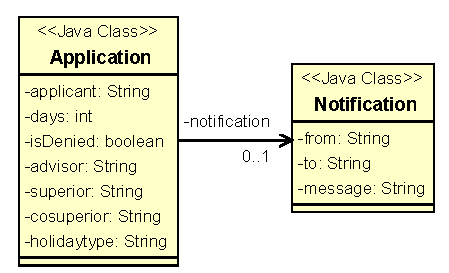
\includegraphics[width=0.5\linewidth]{Bilder/Datenmodell}
\caption{Datenmodell unserer Anwendung}
\label{fig:Datenmodell}
\end{figure}

In der Klasse Application werden alle Daten gespeichert, die für den Urlaubsantrag relevant sind. Neben dem Antragssteller (applicant) werden die Anzahl der Werktage (days) und der Typ des Urlaubs (holidaytype) gespeichert. Außerdem ist der Vorgesetzte (superior), der Stellvertreter (cosuperior) und der zuständige Sachbearbeiter (advisor) hinterlegt. Außerdem speichern wir den Antragsstatus (isDenied) und eine dazugehörige Benachrichtigung (notification), die der Mitarbeiter abschließend erhält.

Die Klasse Notification repräsentiert die Daten für eine Benachrichtigung. Hier werden Absender, Empfänger und die Nachricht hinterlegt. 

\subsubsection{Schnittstellen}

\begin{figure}[H]
\centering
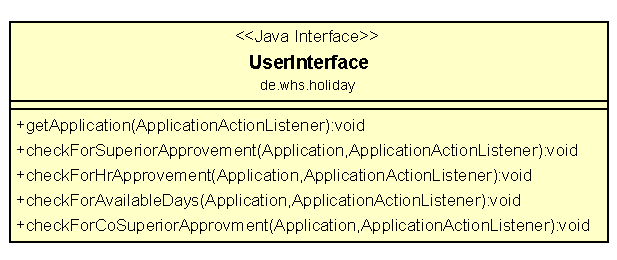
\includegraphics[width=0.7\linewidth]{Bilder/SchnittstelleUserInterface}
\caption{Die Schnittstelle UserInterface}
\label{fig:SchnittstelleUserInterface}
\end{figure}

Abbildung \ref{fig:SchnittstelleUserInterface} zeigt das UserInterface worüber die Interaktion mit dem Endanwender realisiert wird. Die Funktionen repräsentieren dabei die verschiedenen Prozessschritte wie beispielsweise "`Genehmigung durch Vorgesetzten"' oder "`Prüfung ausreichend freier Urlaubstage"'. In unserer Anwendung gibt es zwei Implementierungen für das Interface: Eine Konsolenanwendung und eine GUI die wir in Swing realisiert haben.

\begin{figure}[H]
\centering
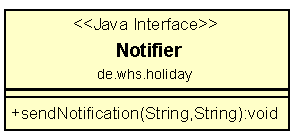
\includegraphics[width=0.35\linewidth]{Bilder/SchnittstelleNotifier}
\caption{Die Schnittstelle Notifier}
\label{fig:SchnittstelleNotifier}
\end{figure}

Zum Verschicken von Benachrichtigungen haben wir die Schnittstelle Notifier (s. Abbildung \ref{fig:SchnittstelleNotifier}) definiert. Für eine reale Unternehmensanwendung könnte man sich hier beispielsweise einen E-Mail-Dienst vorstellen. In unserer Anwendung haben wir die Benachrichtigung über eine Ausgabe in der GUI realisiert.

\begin{figure}[H]
\centering
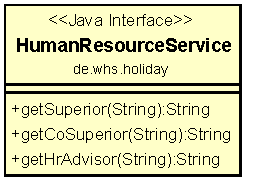
\includegraphics[width=0.3\linewidth]{Bilder/SchnittstelleHumanResourceService}
\caption{Die Schnittstelle HumanResourceService}
\label{fig:SchnittstelleHumanResourceService}
\end{figure}

Abbildung \ref{fig:SchnittstelleHumanResourceService} zeigt die Schnittstelle HumanResourceService, die es uns ermöglicht den Vorgesetzten, Stellvertreter und zuständigen Personalsachbearbeiter für den Antragssteller zu ermitteln. In der Realität könnte man hier beispielsweise das Active-Directory des Unternehmens einbinden. Für unseren Prototyp haben wir die Personalhierarchie unseres Beispielunternehmens statisch hinterlegt.

\subsection{Business Workflow}

Beschreibung der einzelnen Prozessschritte 

\begin{figure}[H]
\centering
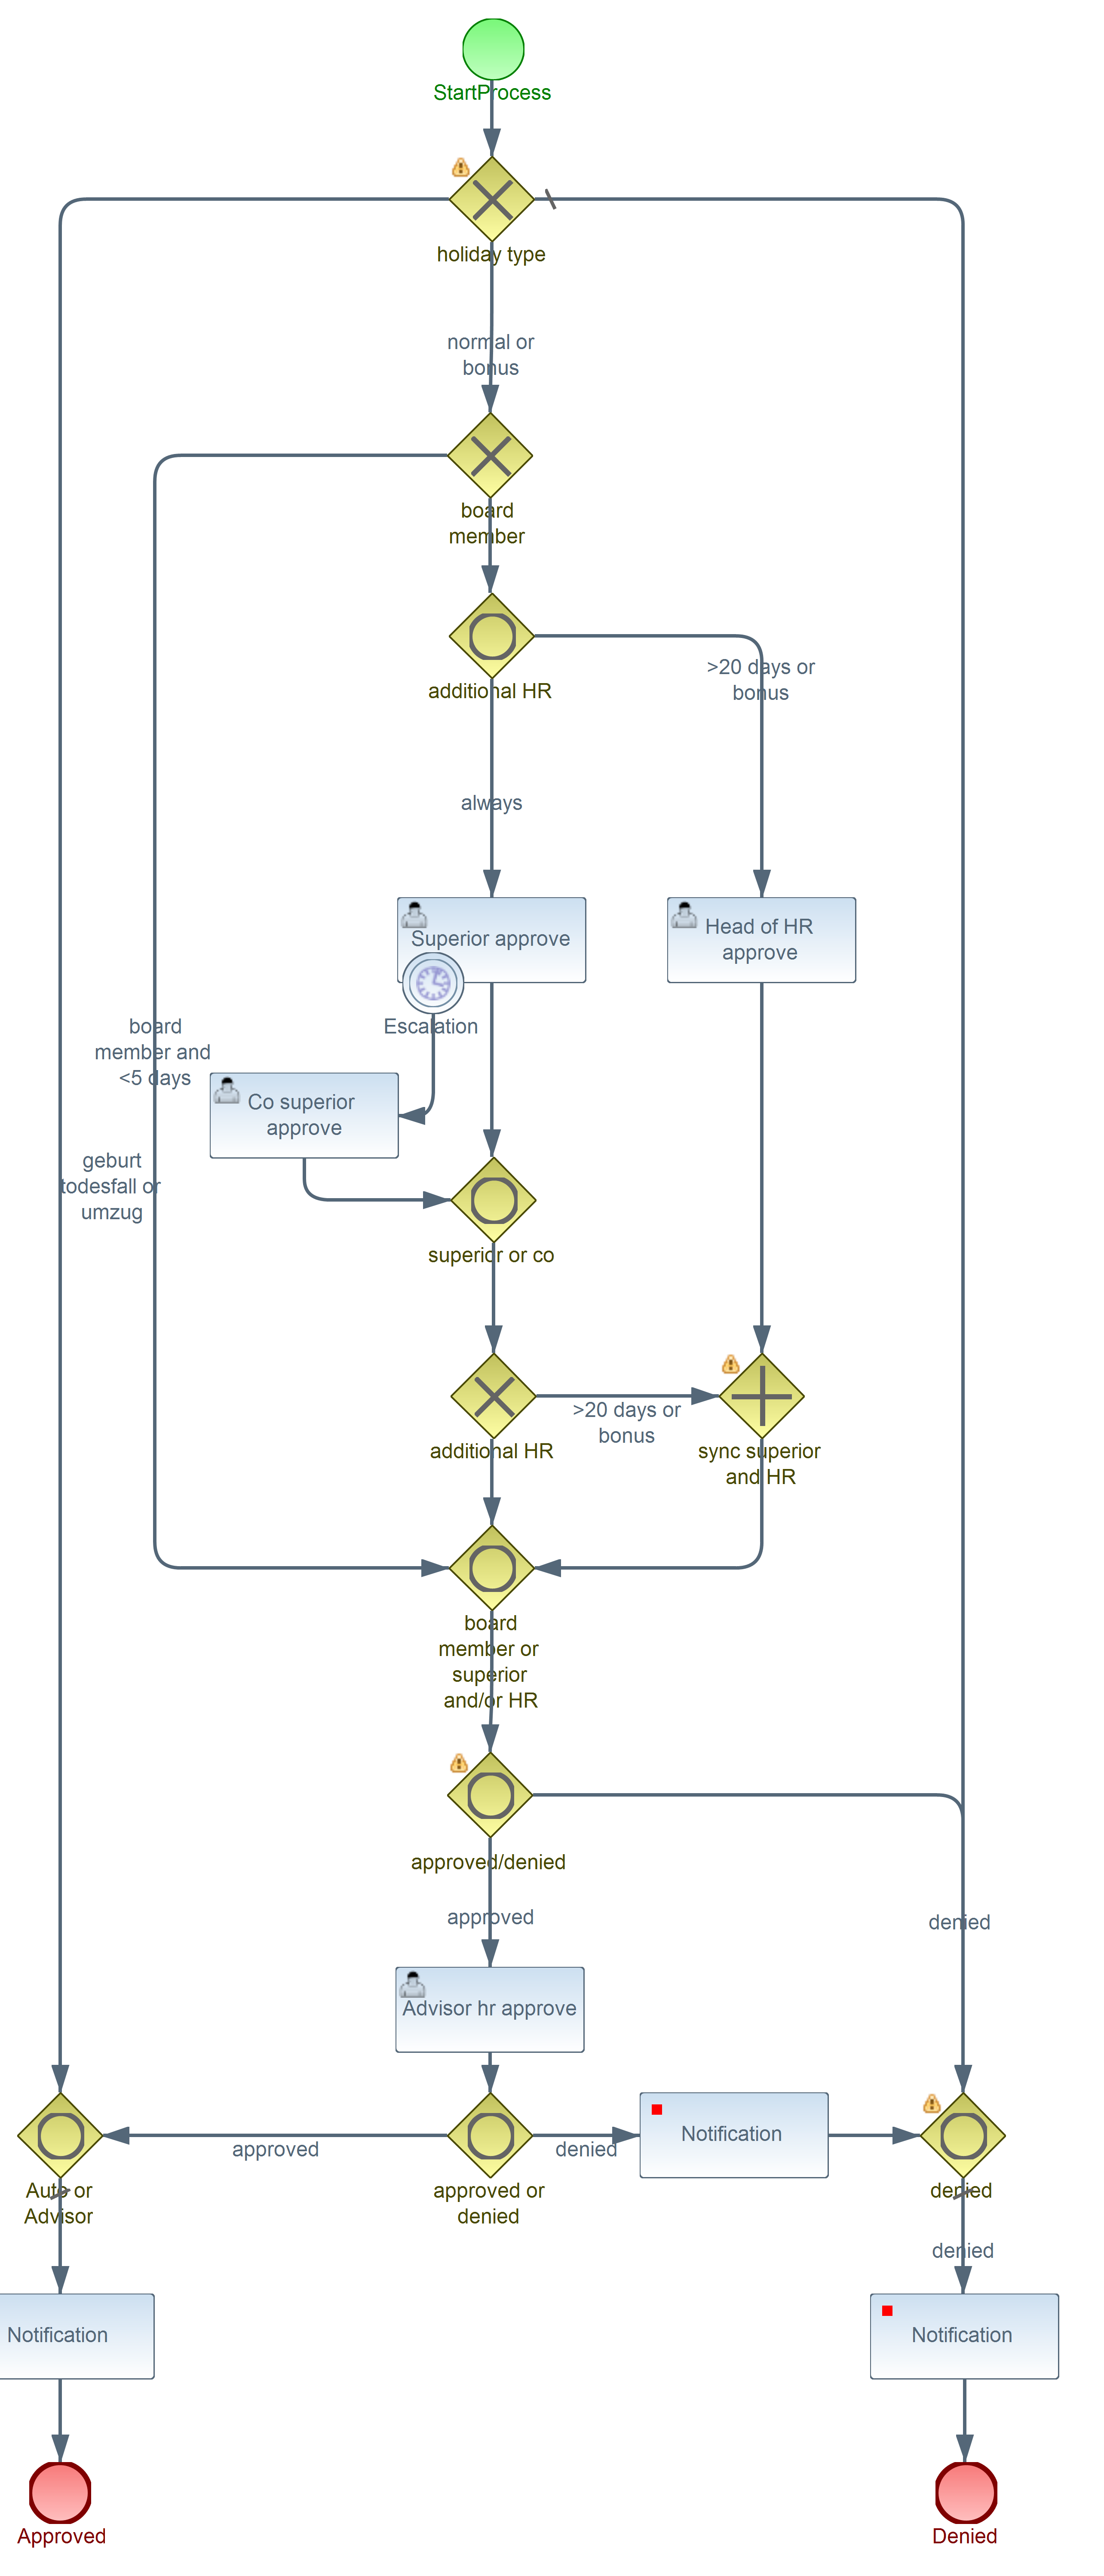
\includegraphics[width=0.75\linewidth]{Bilder/Urlaubsantrag}
\caption{Unser Workflow zur Urlaubsgenehmigung}
\label{fig:Urlaubsantrag}
\end{figure}



\subsection{GUI}